% ============================================================
% Capstone Project Proposal
% Improving Grasp Planning for Mobile Manipulators through
% Coordinated Base-Arm Motion Control
%
% Overleaf-ready. Compile with pdfLaTeX.
% Title page intentionally omitted.
% ============================================================

\documentclass[12pt,a4paper]{article}

\usepackage[T1]{fontenc}
\usepackage[utf8]{inputenc}
\usepackage{lmodern}
\usepackage[margin=1in]{geometry}
\usepackage{amsmath,amssymb}
\usepackage{graphicx}
\usepackage{subcaption}
\usepackage{setspace}
\usepackage{enumitem}
\usepackage{titlesec}
\usepackage[hidelinks]{hyperref}

\graphicspath{{figures/}{images/}}

\onehalfspacing
\setlength{\parindent}{0.5in}
\setlist[itemize]{itemsep=2pt,topsep=4pt}
\setlist[enumerate]{itemsep=2pt,topsep=4pt}

\titleformat{\section}{\normalfont\large\bfseries}{\thesection}{1em}{}
\titleformat{\subsection}{\normalfont\normalsize\bfseries}{\thesubsection}{1em}{}
\titleformat{\subsubsection}{\normalfont\normalsize\itshape}{\thesubsubsection}{1em}{}

% --- Placeholder box for figures that are not yet inserted -------------
% Replace \figplaceholder{...}{...} with \includegraphics when the real
% image files are available.
% \begin{figure}
%     \centering
%     
\includegraphics[width=0.5\linewidth]{chula_logo_thumb.png}
% \end{figure}
\newcommand{\figplaceholder}[2]{%
  \fbox{\begin{minipage}[c][#2][c]{#1}
    \centering \textit{[ Image placeholder ]}
  \end{minipage}}%
}

\begin{document}

% ============================================================
% TITLE PAGE
% ============================================================
\begin{titlepage}
\centering
\thispagestyle{empty}
\vspace*{0.8in}

% ---------------- LOGO PLACEHOLDER --------------------------
% Replace the placeholder below with:
%   \includegraphics[width=0.40\textwidth]{chula_logo.png}
% \figplaceholder{0.40\textwidth}{3cm}
% \begin{figure}
%     \centering
%     
\includegraphics[width=0.5\linewidth]{chula_logo_thumb.png}
% \end{figure}

\includegraphics[width=0.40\textwidth]{chula_logo.jpg}
% ------------------------------------------------------------

\vspace{0.5in}

{\LARGE\bfseries Capstone Project Proposal\par}

\vspace{0.35in}

{\large\bfseries Topic\par}
\vspace{0.10in}
{\large Improving Grasp Planning for Mobile Manipulators through\\
Coordinated Base--Arm Motion Control\par}

\vspace{0.55in}

{\large\bfseries Advisor\par}
\vspace{0.10in}
{\large Assoc.Prof. Ronnapee Chaichaowarat, Ph.D.\par}

\vspace{0.55in}

{\large\bfseries Submitted By\par}
\vspace{0.10in}
{\large
Supphakorn Akkapoo 6638226721\\
Natapol Chusang 6638050521\\
Taratorn Assawadejmetakul 6638087821\par}

\vspace{0.55in}

{\large\bfseries Majors\par}
\vspace{0.10in}
{\large Robotics and Artificial Intelligence Engineering\par}

\vfill
\end{titlepage}

\setcounter{page}{1}

% ============================================================
\section*{Background and Problem Statement}
\addcontentsline{toc}{section}{Background and Problem Statement}

Mobile manipulators combine the mobility of a mobile platform with the dexterity of a robotic arm, making them suitable for tasks such as object grasping and manipulation in
unstructured environments. However, motion planning for these systems is challenging because
the mobile base and manipulator are often treated as separate components. In a conventional
sequential approach, the robot first moves its mobile base to a predefined position near the
target object, after which the robotic arm plans and executes the grasping trajectory~[1].

Although this approach simplifies the planning process, it can cause the manipulator to
begin from an unfavorable configuration. The resulting arm trajectory may encounter obstacles,
self-collisions, joint limits, or kinematic singularities. Furthermore, the mobile base must reach a
sufficiently precise position and orientation for the arm to successfully reach the target, which
can limit the robot's ability to adapt to different object locations and environmental conditions.
Selecting a base position from which the target is reachable has long been treated as a distinct
sub-problem, addressed with reachability and capability maps~[1].

Recent advances in domestic service robotics have introduced technologies that can
improve different stages of the manipulation pipeline. Learned 6-DoF grasp generators can
generate grasp candidates from visual observations using models trained on millions of
simulated grasps~[4],~[5]. In parallel, GPU-accelerated motion planning methods can generate
collision-free robot trajectories efficiently, enabling more computationally demanding planning
approaches to be considered for practical robotic systems~[3]. Open-vocabulary perception
models can further detect and segment objects from free-form text prompts, providing more
flexible target-object identification in unstructured environments~[6].

With recent advances in whole-body motion planning, robotic systems can instead
coordinate the motion of the mobile base and manipulator as a single system~[1],~[2]. This
allows the mobile base to contribute to achieving the desired end-effector pose rather than
requiring the base to first reach a fixed predefined position.

At the same time, advances in Vision-Language-Action (VLA) models have introduced
new approaches for robotic manipulation by enabling robots to use visual and language
information to generate robot actions and improve generalization across tasks and
environments~[7]--[10]. This approach, however, comes with a significant cost in both monetary
and computational resources. This raises the question on whether the performance increase
from VLAs are worth the resource trade-offs that a traditional manipulation model would not
have to make.

\newpage 
Therefore, this project investigates two distinct approaches to improving grasp planning
for mobile manipulators. The first is a classical model-based approach, which combines the
kinematic models of the mobile base and manipulator into a unified whole-body model and
coordinates their motion during grasp planning. The second is an AI-based approach using VLA
models, which investigates whether a learned model can reason about the environment, target
object, and manipulation task to generate appropriate actions.

The key problem addressed by this project is determining how these two fundamentally
different approaches can improve mobile-manipulator grasping, and how their performance
differs under varying object and environmental conditions.

% ============================================================
\section*{Objective}
\addcontentsline{toc}{section}{Objective}

The primary objective of this project is to investigate and compare two approaches for
improving grasp planning in mobile manipulators: classical coordinated base--arm motion
planning and Vision-Language-Action (VLA)-based planning.

The specific objectives are:

\begin{enumerate}
  \item Develop a unified kinematic model of the mobile base and robotic arm that allows both
        systems to be considered simultaneously during grasp planning.
  \item Develop a coordinated base--arm motion planning approach that enables the mobile
        base and manipulator to contribute jointly toward achieving a desired grasp pose while
        considering constraints such as collision, joint limits, and kinematic singularities.
  \item Investigate a VLA-based grasp-planning approach capable of using visual and task-related
        information to generate appropriate actions for mobile-manipulator grasping.
  \item Evaluate the two approaches independently under different object positions,
        environmental configurations, and manipulation scenarios.
  \item Compare the performance of the classical and VLA approaches using metrics such as
        grasp success rate, trajectory efficiency, execution time, robustness, collision occurrence,
        and adaptability to different conditions.
  \item Identify the advantages, limitations, and appropriate applications of each approach for
        practical mobile-manipulator grasping systems.
\end{enumerate}

% ============================================================
\section*{Literature Review}
\addcontentsline{toc}{section}{Literature Review}

\subsection*{Motion Planning for Mobile Manipulators}

Mobile manipulators combine the mobility of a mobile base with the dexterity of a
robotic arm. This additional degree of freedom provides a larger reachable workspace, but also
makes motion planning more complex because the base and manipulator are kinematically
coupled. A systematic review by Su\'arez-Ruiz et al. classifies mobile-manipulator motion
planning approaches into several categories and highlights the importance of selecting an
appropriate base configuration to ensure that the target remains within the manipulator's
reachable workspace. Conventional approaches frequently determine a suitable base position
first and subsequently plan the manipulator trajectory. While this decouples the planning
problem and simplifies implementation, it can restrict the available grasp configurations and
may result in inefficient or infeasible arm trajectories~[1].

More recent work has investigated whole-body motion planning, where the mobile
base and manipulator are represented as a single system. Kim et al. proposed a nonlinear model
predictive control (NMPC) approach for whole-body motion planning of an omnidirectional
mobile manipulator. Their system modeled the mobile base and six-degree-of-freedom arm as a
unified nine-degree-of-freedom system and incorporated collision avoidance into the
optimization process. The method was able to track an end-effector pose while simultaneously
avoiding self-collision and environmental obstacles~[2].

This approach is particularly relevant to the proposed project because it demonstrates
that the mobile base does not necessarily need to reach a fixed grasping position before arm
motion begins. Instead, base motion can be treated as an additional set of degrees of freedom
that contributes to achieving the desired end-effector pose.

Current robotic software frameworks also support this concept. For example, MoveIt
provides mechanisms for planning coordinated motion between a mobile base and manipulator,
while recommending Nav2 for navigation-only tasks. This demonstrates the increasing
availability of practical tools for integrating base and arm motion within a common planning
framework.

However, existing whole-body approaches generally focus on generating feasible or
collision-free motion rather than specifically investigating how coordinated base--arm motion
affects grasp success and grasp quality~[1],~[2]. Therefore, there remains an opportunity to
investigate base--arm coordination specifically as a grasp-planning strategy and to evaluate its
effect under different object positions and environmental constraints.

\newpage
\subsection*{6-DoF Grasp Generation}

In addition to determining how the robot should move, a mobile manipulator must
determine an appropriate grasp pose for the target object. Learning-based grasp generation has
become an important research direction because it allows robots to generate grasp candidates
directly from visual observations.

Contact-GraspNet introduced an efficient approach for generating 6-DoF parallel-jaw
grasp distributions directly from scene depth data. Instead of representing the complete grasp
pose independently, the method associates grasp configurations with points in the observed
point cloud, reducing the effective representation dimensionality. The model was trained using
17 million simulated grasps and demonstrated more than 90\% success in experiments involving
unseen objects in structured clutter~[4].

More recently, GraspGen investigated diffusion-based grasp generation. The method
models grasp generation as an iterative diffusion process and combines a Diffusion Transformer
with a discriminator for ranking generated grasp candidates. The authors generated more than
53 million simulated grasps and demonstrated generalization across different objects, grippers,
and observation conditions. GraspGen also reports real-time inference at approximately 20~Hz
before TensorRT optimization and state-of-the-art performance on the FetchBench grasping
benchmark~[5].

These developments show that modern grasp planning can generate multiple candidate
6-DoF grasp poses from visual information rather than relying on manually defined grasp
positions. However, grasp generation alone does not guarantee that a mobile manipulator can
physically reach the selected grasp. A grasp pose may be valid for the end-effector but
unreachable from the current arm and base configuration, or it may result in collisions or
unfavorable joint configurations.

Therefore, grasp generation and whole-body motion planning should be considered
complementary problems. In the proposed project, generated grasp poses can serve as target
configurations, while the coordinated base--arm planner determines how the mobile
manipulator should move to reach those configurations.

\subsection*{Motion Optimization and Collision-Free Planning}

Once a target grasp pose has been generated, the robot must produce a collision-free
trajectory from its current configuration to the target. GPU-accelerated motion planning has
recently improved the computational efficiency of this process~[3].

cuRobo formulates robot motion generation as a global optimization problem and uses
massively parallel GPU computation to evaluate multiple optimization seeds simultaneously.
The system combines trajectory optimization, geometric planning, and collision-free inverse
kinematics. The authors report average motion-generation times of approximately 53~ms for
difficult planning problems and significantly faster performance than conventional
trajectory-optimization and sampling-based planning approaches.

This type of accelerated motion generation is particularly relevant for mobile
manipulators because whole-body planning increases the dimensionality of the configuration
space. For Walkie~4, incorporating the mobile base together with a 7-DoF manipulator creates a
higher-dimensional planning problem than conventional fixed-base manipulation. Efficient
collision checking and trajectory optimization are therefore important for achieving practical
execution times.

The proposed project can use these developments as a technical foundation for the
classical approach. Instead of planning an arm trajectory after the base reaches a predefined
pose, the base degrees of freedom can be incorporated into the planning problem. The planner
can then optimize the combined configuration while considering collision avoidance, joint limits,
and the desired end-effector pose.

\subsection*{Open-Vocabulary Perception for Manipulation}

Modern manipulation systems increasingly require robots to identify objects that were
not explicitly defined during system development. YOLOE addresses this problem through
open-vocabulary object detection and segmentation. Rather than restricting the model to a
fixed set of predefined object categories, YOLOE supports text prompts, visual prompts, and
prompt-free detection within a unified model. The ICCV 2025 results demonstrate strong
zero-shot transfer performance while maintaining real-time inference efficiency~[6].

Open-vocabulary perception is relevant to the proposed VLA approach because it
provides a mechanism for identifying task-relevant objects from natural-language descriptions.
For example, a command such as ``pick up the bottle'' can be converted into visual information
that identifies the target object. This perception capability can then be combined with grasp
generation and robot action planning.

However, object detection and segmentation alone do not determine how the mobile
manipulator should move. They provide information about the target, but a separate planning
or policy layer is still required to determine the appropriate base, arm, and gripper actions.

\newpage
\subsection*{Vision-Language-Action Models}

Vision-Language-Action models represent a shift from manually designed perception
and planning pipelines toward learned policies that directly connect visual observations,
language instructions, and robot actions. RT-2 demonstrated an early influential approach by
fine-tuning vision-language models with robot trajectory data while representing robot actions
as tokens within the same model. The resulting system demonstrated improved generalization
to novel objects and the ability to perform manipulation tasks based on semantic instructions~[7].

Subsequent work has focused on developing general-purpose robot policies that can
transfer across tasks and robot embodiments. Octo is a large transformer-based robot policy
trained on approximately 800,000 trajectories from the Open X-Embodiment dataset. It can
receive language commands or goal images and can be fine-tuned to new sensory inputs and
action spaces. Experiments across nine robotic platforms demonstrate the potential for
pretrained policies to reduce the amount of task-specific training required for new robotic
systems~[8].

Recent surveys indicate that VLA research is rapidly expanding toward general-purpose
manipulation. Kawaharazuka et al. describe VLA models as systems that combine visual,
language, and action information to learn policies capable of generalizing across tasks, objects,
robot embodiments, and environments. Their review covers model architectures, training
strategies, datasets, robot platforms, and evaluation methods for real-world deployment~[9].

A separate systematic review by Ud Din et al. analyzed 102 VLA models, 26 foundational
datasets, and 12 simulation platforms, highlighting the rapid development of VLA-based robotic
manipulation and the remaining challenges in scalable training, multimodal alignment, and
real-world deployment~[10].

Despite their potential for generalization, VLA models introduce different challenges
from classical motion planning. Their performance depends heavily on the training data, robot
embodiment, observation modality, and action representation. Furthermore, a learned policy
may generate actions that are semantically appropriate but violate physical constraints such as
joint limits, collisions, or workspace limitations. These issues make direct comparison between
classical and VLA approaches particularly relevant~[7]--[10].

% ============================================================
\newpage
\section*{Research Gap}
\addcontentsline{toc}{section}{Research Gap}

The literature demonstrates substantial progress in both classical whole-body motion
planning and learning-based robotic manipulation. Classical approaches provide explicit
representations of robot kinematics and physical constraints, allowing collision avoidance, joint
limits, and end-effector constraints to be directly incorporated into the planning problem.
Whole-body approaches additionally allow the mobile base to contribute to manipulation
rather than treating navigation and grasping as independent stages~[1],~[2],~[3].

In parallel, learning-based methods have substantially improved grasp generation and
high-level manipulation. Contact-GraspNet and GraspGen demonstrate that learned models can
generate effective 6-DoF grasp candidates from visual observations, while VLA models such as
RT-2 and Octo demonstrate the potential to map multimodal observations and task instructions
to robot actions~[4],~[5],~[7],~[8].

However, these two research directions address different levels of the manipulation
problem. Grasp-generation methods primarily determine where and how to grasp, while
whole-body motion planners determine how the robot can physically reach the desired pose.
VLA models attempt to integrate perception, reasoning, and action, but their behavior is
learned rather than explicitly constrained by the robot's kinematic model~[1],~[4],~[5],~[7]--[10].

Therefore, this project proposes a direct comparison between two fundamentally
different approaches to mobile-manipulator grasp planning:

\begin{itemize}
  \item \textbf{Classical model-based approach:} construct a unified mobile-base and manipulator
        kinematic model and jointly optimize their motion toward a desired grasp pose while
        explicitly considering physical constraints.
  \item \textbf{VLA-based approach:} use visual and task-level information to generate appropriate
        manipulation actions through a learned policy.
\end{itemize}

The comparison will focus not only on grasp success but also on trajectory efficiency, execution
time, collision occurrence, robustness, and adaptability to different object and environmental
configurations. This comparison is intended to clarify the trade-offs between explicit
model-based planning and learned multimodal action generation for practical
mobile-manipulator grasping.

% ============================================================
\newpage
\section*{Methodology}
\addcontentsline{toc}{section}{Methodology}

\subsection*{Project Background}

This capstone project is conducted as an extension of an existing mobile-manipulator
platform named \textbf{Walkie}, developed by the \textbf{Engineer Innovator Club (EIC)} at Chulalongkorn
University for participation in the RoboCup@Home competition. EIC is a student engineering
organization that develops robotic systems for national and international robotics competitions.
The Walkie project was initiated in September 2025 and has been continuously developed
through collaboration among students from multiple engineering disciplines, including
mechanical, electrical, software, and artificial intelligence teams.

% ---------------- FIGURE PLACEHOLDER 1 ----------------------

    
    \begin{center}
        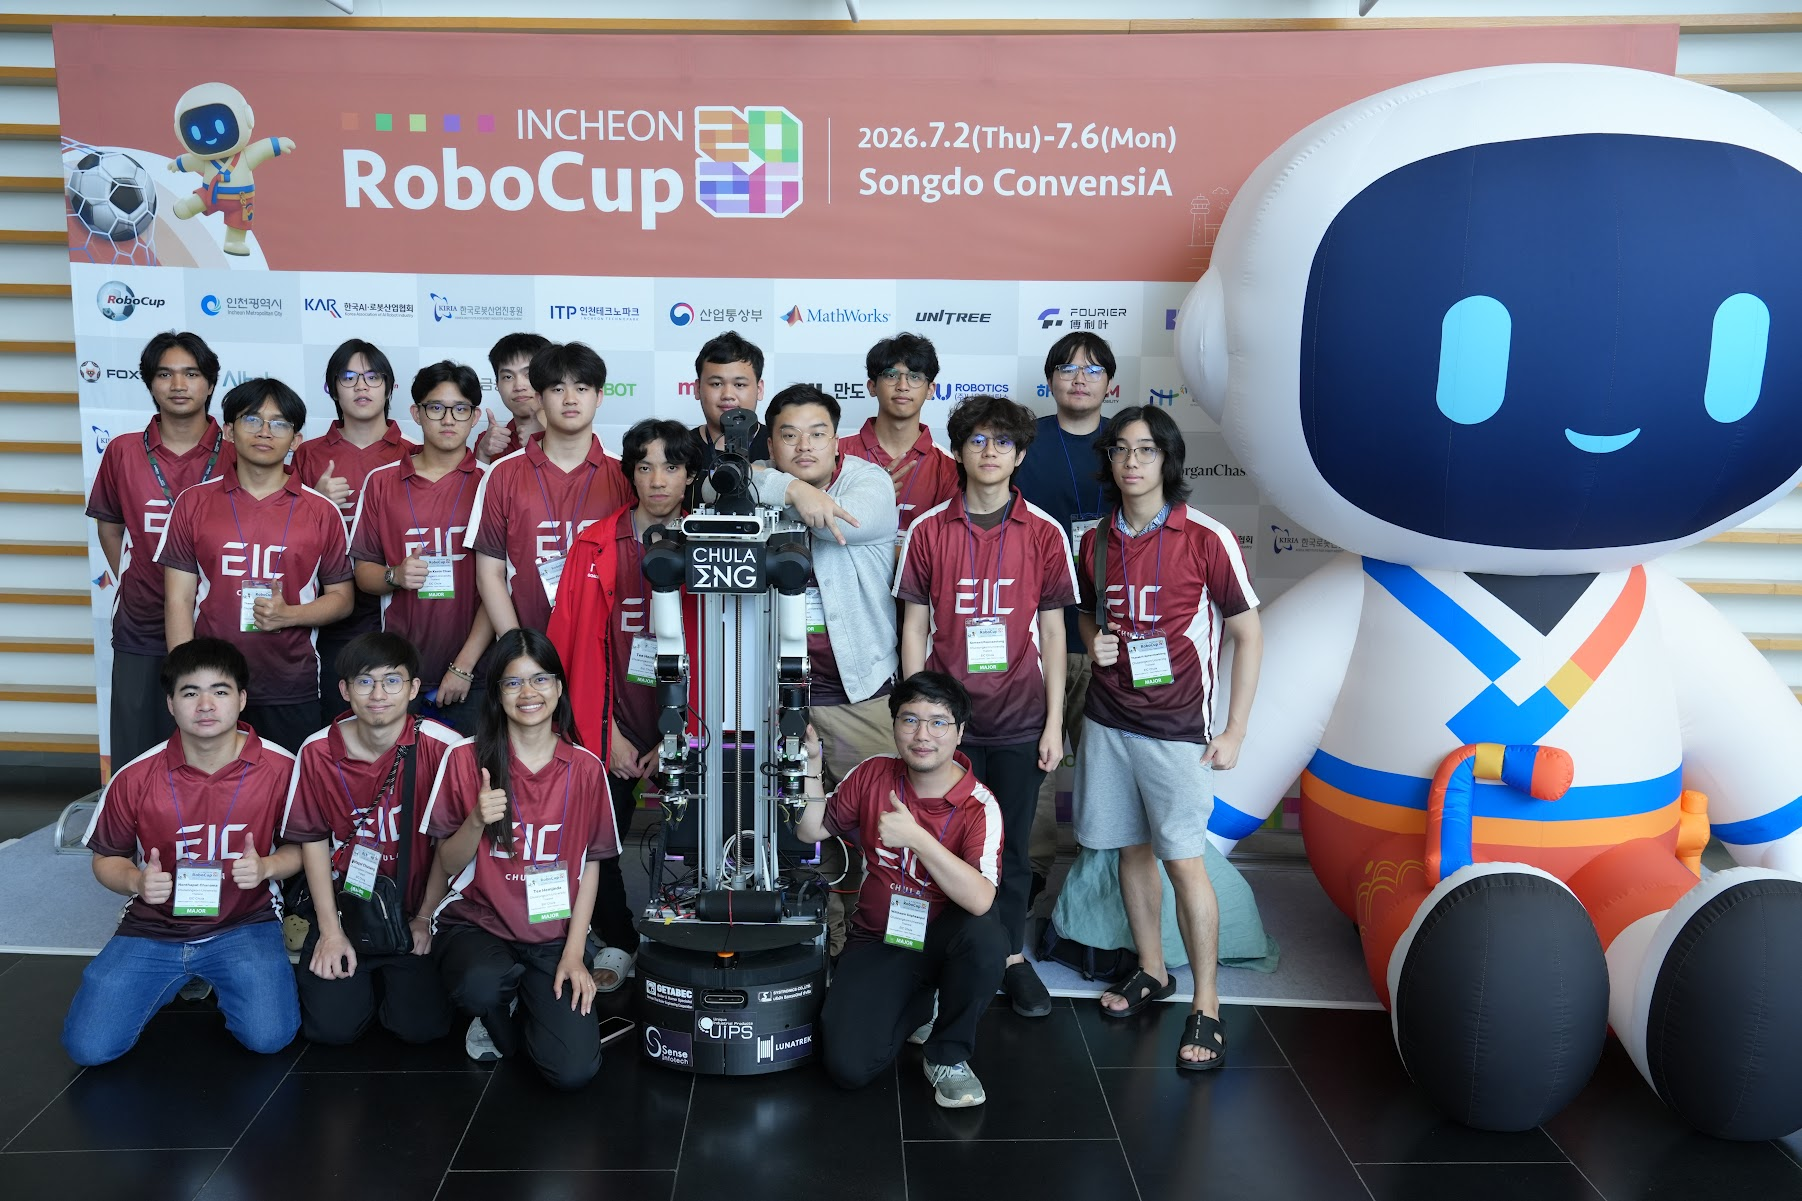
\includegraphics[width=0.75\linewidth]{DSC06194.jpg}
        \\ \small{\textit{{Walkie and EIC RoboCup@Home Team}}}
    \end{center}


% ------------------------------------------------------------

The three members of this capstone project have also been directly involved in the
development of Walkie since the previous project year, allowing the proposed research to build
upon an existing system and accumulated technical experience. During the previous year,
\textbf{Supphakorn Akkapoo} served as Head of the Mechanical Department, \textbf{Taratorn
Assawadejmetakul} served as President of EIC RoboCup@Home project, and \textbf{Natapol Chusang}
worked as a member of the Software Integration Team. In the current project year, Supphakorn
serves as President of EIC RoboCup@Home project, Taratorn is working with the AI Team on
VLA Project, and Natapol continues to work with the Software Integration Team. This continuity
provides the team with direct knowledge of the robot's mechanical design, software
architecture, integration process, and previous development decisions.

\newpage
Walkie is an autonomous mobile service robot designed to perform household and
human-assistance tasks. Unlike a conventional fixed-base robotic manipulator, Walkie combines
a mobile omnidirectional drivebase with a robotic arm, allowing it to both navigate through an
environment and physically interact with objects. The robot was developed for
RoboCup@Home, an international robotics competition focused on autonomous service robots
operating in domestic environments. Tasks in this competition require capabilities including
autonomous navigation, object recognition, manipulation, and interaction with people.

The current Walkie platform consists of a four-wheel omnidirectional drivebase, a
vertically actuated lift mechanism, and 2 humanoid 7-DOF OpenArm robotic manipulators.
The omnidirectional drivebase provides planar movement and rotation, while the lift
mechanism provides additional vertical positioning and increases the manipulator's reachable
workspace. The OpenArm provides the dexterity required for object manipulation and grasping.
A custom mounting platform was developed to integrate the OpenArm with the lift and mobile
platform.

% ---------------- FIGURE PLACEHOLDER 2 (optional) -----------
% Additional platform photograph or CAD render can be inserted here.
% \begin{figure}[htbp]
%   \centering
%   \figplaceholder{0.7\textwidth}{6cm}
%   % \includegraphics[width=0.7\textwidth]{walkie_platform.jpg}
%   \caption*{\textit{Walkie platform overview}}
% \end{figure}
% ------------------------------------------------------------

Walkie has undergone approximately one year of development involving mechanical
design, manufacturing, electrical integration, software development, and system testing. The
project initially focused on the development of the omnidirectional drivebase and subsequently
progressed to the development of custom robotic arms. Two generations of an in-house robotic
arm were designed and tested before the team transitioned to the OpenArm platform to
improve reliability and reduce development risk prior to the competition. The existing system
was subsequently integrated with ROS~2, Nav2 and MoveIt for robot control and
motion-planning development.

Following completion of the major mechanical systems, Walkie underwent extensive
system-level testing and scenario-based trials in preparation for RoboCup@Home 2026. The
robot was eventually deployed at the competition in Songdo, Incheon, South Korea, where the
team competed against 24 international teams and achieved 6th place.

This previous development provides the proposed capstone project with an existing
physical platform, established mechanical dimensions, known actuator and sensor interfaces, an
existing software environment, and practical knowledge of the robot's limitations.
Consequently, the project does not aim to construct a new mobile manipulator or redesign the
existing Walkie hardware. Instead, the research will focus on improving the motion-planning
and grasp-planning capabilities of the existing platform.

Although Walkie is already capable of performing autonomous manipulation tasks, its
development has primarily focused on achieving reliable system performance for competition
scenarios. The proposed project therefore addresses a different problem: determining whether
the mobility of the robot can be more effectively incorporated into grasp planning. In a
conventional sequential approach, the mobile base first moves to a selected position near the
target, after which the manipulator performs the grasp. Such an approach can unnecessarily
constrain the arm configuration and may result in inefficient or infeasible grasp trajectories.

This project proposes to investigate an alternative approach in which the mobile base,
lift, and manipulator are considered as a \textbf{coordinated system} during grasp planning. By
allowing the base to actively contribute to the positioning of the end-effector, the robot may be
able to reach a grasp pose that is difficult or impossible to achieve using arm-only motion from
a fixed base configuration.

Therefore, the methodology focuses on developing and evaluating a coordinated
mobile-manipulator motion-planning framework for the existing Walkie platform. The work will
begin by developing a simulation model and unified kinematic representation of Walkie.
Classical approaches such as whole-body inverse kinematics and optimization-based planning
will then be investigated and compared against a conventional sequential planning baseline.
Following successful validation of the classical approach, learned 6-DoF grasp generation
methods may be integrated to investigate the interaction between grasp selection and
whole-body reachability. Finally, the most promising approach will be transferred from
simulation to the physical Walkie robot for sim-to-real validation.

\subsection*{System Characterization}

Before developing the proposed planning framework, the existing Walkie platform will
be characterized to obtain the parameters required for simulation and kinematic modeling. The
robot's physical dimensions, coordinate frames, joint limits, lift range, manipulator geometry,
end-effector configuration, and mobile-base kinematics will be documented from the existing
CAD models, robot configuration files, and physical measurements. These parameters will be
used to construct a consistent representation of Walkie across the simulation and physical
robot.

The existing ROS~2 and MoveIt configuration will serve as the initial software reference
because these frameworks have already been used for robotic-arm integration and
motion-planning tests during the development of Walkie. The resulting system description will
define the interfaces between the mobile base, lift, manipulator, and end-effector and will
provide the parameters required for the unified kinematic model developed in the subsequent
stage.

\subsection*{Simulation Environment Development}

A digital simulation model of Walkie will then be developed using either NVIDIA Isaac
Sim or Gazebo. The simulator will be selected based on compatibility with the robot model,
motion-planning framework, perception modules, and available computational resources.

The simulation will reproduce the major components relevant to manipulation, including
the omnidirectional mobile base, vertical lift, 7-DOF manipulator, gripper, and relevant collision
geometry. Configurable objects and obstacles will also be added to represent different
manipulation environments.

The simulated model will be validated against the physical Walkie platform using basic
geometric and kinematic tests. These tests will include joint-range verification, lift motion, base
motion, and end-effector pose validation.

% ---------------- FIGURE PLACEHOLDER 3 (optional) -----------
% Simulation environment screenshot.
% \begin{figure}[htbp]
%   \centering
%   \figplaceholder{0.8\textwidth}{6cm}
%   % \includegraphics[width=0.8\textwidth]{simulation_env.png}
%   \caption*{\textit{Simulation environment}}
% \end{figure}
% ------------------------------------------------------------

Once validated, the simulation will serve as the primary environment for algorithm
development and controlled experimentation before transferring the most successful approach
to the physical robot.

\subsection*{Unified Mobile-Manipulator Kinematic Model~[1],~[2]}

The mobile base, lift, and robotic arm will be modeled as a single kinematic system rather than
as independent subsystems.

The generalized configuration of Walkie can be represented as

\begin{equation}
q = \begin{bmatrix} x_b & y_b & \theta_b & z_l & q_1 & q_2 & \cdots & q_7 \end{bmatrix}^{T}
\end{equation}

where $x_b$, $y_b$, and $\theta_b$ represent the position and orientation of the mobile base, $z_l$ represents
the lift position, and $q_1, q_2, \ldots, q_7$ represent the joint positions of the OpenArm.

Thus, the transformation

\begin{equation}
{}^{W}T_{E} = {}^{W}T_{B}\, {}^{B}T_{L}\, {}^{L}T_{A}\, {}^{A}T_{E}
\end{equation}

Here $W$, $B$, $L$, $A$, and $E$ represent the coordinate frames used to describe the different parts of
Walkie:

\begin{itemize}
  \item $W$ = World frame: the fixed reference frame of the environment.
  \item $B$ = Base frame: the coordinate frame attached to Walkie's mobile drivebase.
  \item $L$ = Lift frame: the coordinate frame attached to the vertical lift.
  \item $A$ = Arm frame: the coordinate frame attached to the base of the OpenArm manipulator.
  \item $E$ = End-effector frame: the coordinate frame attached to the gripper.
\end{itemize}

and the corresponding Jacobian will describe the contribution of both mobile-base and
manipulator motion to the end-effector:

\begin{equation}
\dot{x} = J(q)\,\dot{q}
\end{equation}

The objective of this unified model is to allow Walkie's base motion, lift motion, and arm
motion to be considered simultaneously during grasp planning. This changes the planning
problem from a sequential base-then-arm process to a coordinated whole-body problem in
which the base can actively contribute to reaching the desired grasp pose.

\subsection*{Baseline Sequential Motion Planning~[1]}

A conventional sequential planning strategy will first be implemented as a baseline.
The target object will be assigned a suitable base position, after which Walkie will navigate to
the selected position. Once the base reaches the target configuration, it will remain stationary
while the manipulator independently plans and executes a trajectory toward the grasp pose.

This baseline will provide a reference against which the proposed coordinated planning
methods can be evaluated. The same target objects, initial configurations, and environmental
conditions will be used for both approaches.

\subsection*{Classical Coordinated Base--Arm Motion Planning}

The first proposed planning approach will use the unified mobile-manipulator model to
coordinate the motion of the base and manipulator.

\subsubsection*{1. Whole-Body Inverse Kinematics~[1],~[2]}

Whole-body inverse kinematics will first be investigated as a relatively simple
coordinated planning method. The planner will determine a combination of base, lift, and arm
motion required to achieve a desired end-effector pose.

A Jacobian-based formulation may be used:

\begin{equation}
\dot{q} = J^{\dagger}(q)\,\dot{x}
\end{equation}

Additional objectives such as joint-limit avoidance, collision avoidance, trajectory smoothness,
and unnecessary base movement will be incorporated where appropriate.

The primary purpose of this stage is to determine whether the additional degrees of freedom
provided by the mobile base and lift improve the robot's ability to reach target grasp poses
compared with arm-only planning.

\subsubsection*{2. Optimization-Based Planning and NMPC~[2],~[3]}

If the whole-body IK approach demonstrates successful coordinated motion, more advanced
optimization-based approaches will be investigated. In particular, nonlinear model predictive
control (NMPC) will be considered for generating coordinated trajectories while explicitly
considering robot constraints.

The planning problem will optimize a sequence of robot configurations subject to constraints
such as joint limits, velocity limits, collision avoidance, and end-effector pose requirements. A
representative objective function can be expressed as

\begin{equation}
J = w_1 J_{pose} + w_2 J_{collision} + w_3 J_{joint} + w_4 J_{smooth} + w_5 J_{base}
\end{equation}

where $J$ represents the overall cost of the planned motion, and each $J$ term represents a
specific objective:

\begin{itemize}
  \item $J_{pose}$: End-effector pose error, measuring how far the robot's end-effector is from the
        desired grasp position and orientation. A lower value means the robot reaches the
        target pose more accurately.
  \item $J_{collision}$: Collision cost, penalizing trajectories that bring the robot close to or into
        collision with obstacles or other parts of the robot. A higher penalty is assigned to
        unsafe configurations.
  \item $J_{joint}$: Joint-limit cost, penalizing configurations that approach or exceed the allowable
        joint limits. This encourages the robot to remain within a comfortable and feasible range
        of motion.
  \item $J_{smooth}$: Trajectory smoothness cost, penalizing sudden changes in joint or base motion.
        This encourages smoother and more stable trajectories.
  \item $J_{base}$: Base-motion cost, penalizing unnecessary movement of the mobile base. This can
        encourage the planner to use the base only when its additional motion provides a useful
        advantage for reaching the grasp pose.
\end{itemize}

The parameters $w_1, w_2, \ldots, w_5$ are weighting factors that determine the relative importance
of each objective. For example, increasing $w_2$ places greater importance on collision avoidance,
while increasing $w_5$ discourages unnecessary movement of the mobile base.

Although the objective function is expressed as a weighted sum, the optimization problem is
nonlinear because the end-effector pose, collision distances, and robot motion constraints are
nonlinear functions of the robot configuration.

The final selection of the classical planning method will be based on experimental performance,
computational requirements, and implementation feasibility.

\subsection*{Learned 6-DoF Grasp Generation~[4],~[5]}

After the classical coordinated-planning framework has been established, a learned
grasp-generation method will be investigated.

The perception system will identify the target object and provide visual or geometric
information to a 6-DoF grasp-generation model. Methods such as Contact-GraspNet or
GraspGen will be considered for generating candidate grasp poses.

The grasp generator will produce multiple candidate configurations:

\begin{equation}
G = \{\, g_1, g_2, \ldots, g_n \,\}
\end{equation}

Rather than directly executing the first generated grasp, each candidate will be evaluated using
the unified mobile-manipulator model. This allows grasp generation and whole-body
reachability to be considered together.

\subsection*{Integrated Grasp and Whole-Body Planning~[1],~[4],~[5]}

For each generated grasp candidate, the whole-body planner will determine whether Walkie
can physically reach the corresponding end-effector pose while satisfying its kinematic and
collision constraints.

Candidates that cannot be reached, cause collisions, violate joint limits, or produce unsuccessful
trajectories will be rejected.

Feasible candidates can then be ranked according to a combined cost function such as

\begin{equation}
J_i = \alpha_1 J_{grasp,\,i} + \alpha_2 J_{trajectory,\,i} + \alpha_3 J_{base,\,i}
      + \alpha_4 J_{collision,\,i} + \alpha_5 J_{joint,\,i}
\end{equation}

This stage investigates an important aspect of the proposed research: a grasp that appears
suitable from the object perspective may not be the best grasp for the complete mobile
manipulator. The optimal grasp should therefore consider both the quality of the grasp and the
robot's ability to reach and execute it efficiently.

\subsection*{Experimental Scenarios}

The proposed approaches will be tested under controlled simulation scenarios involving
different object positions and environmental configurations.

Object locations will be varied across the robot's workspace, including positions near the robot,
lateral positions, and locations close to the limits of the arm-only workspace. Additional
obstacles will be introduced to create constrained and cluttered environments.

Where applicable, object orientations and different target objects will also be varied to evaluate
the adaptability of the planning methods.

All planning methods will be evaluated using the same initial robot configurations and test
environments to ensure that the comparison is consistent.

\subsection*{Performance Evaluation}

The effectiveness of each method will be evaluated quantitatively.

The primary metric will be grasp success rate:

\begin{equation}
\text{Success Rate} = \frac{N_{successful\ grasps}}{N_{total\ trials}} \times 100\%
\end{equation}

Additional metrics will include planning time, execution time, trajectory length, base
displacement, collision occurrence, planning failure rate, and robustness across different object
and environmental configurations.

Repeated trials will be conducted for each test condition. The resulting measurements will be
summarized using appropriate statistical measures such as mean and standard deviation.

The key comparison will determine whether coordinated base--arm planning provides
measurable improvements over conventional sequential planning and under which
environmental conditions the improvements are most significant.

\subsection*{Sim-to-Real Validation~[4],~[5],~[8]}

Following successful simulation experiments, the most promising planning approach will be
transferred to the physical Walkie platform.

The sim-to-real evaluation will initially use controlled conditions with known target positions
and simple environments. Once reliable operation has been established, perception-based
target localization and learned grasp generation will be introduced.

The validation process will therefore progress from simulation to increasingly realistic physical
experiments:

\begin{equation*}
\textit{Simulation} \rightarrow \textit{Real Walkie / Known Target} \rightarrow
\textit{Real Walkie / Perception} \rightarrow \textit{Real Walkie / Learned Grasp}
\end{equation*}

Performance differences between simulation and physical execution will be analyzed to identify
the effects of modeling inaccuracies, mechanical tolerances, actuator limitations, perception
errors, and other real-world factors.

\subsection*{Overall Methodology~[1]--[5]}

The proposed methodology follows a progressive development strategy built around the
existing Walkie platform. Rather than developing a new robot, the project will first establish an
accurate simulation and unified kinematic representation of the existing system. A conventional
sequential base-then-arm strategy will then be used as a baseline, followed by increasingly
sophisticated coordinated approaches based on whole-body inverse kinematics and
optimization-based planning.

Once the classical framework has been validated, learned 6-DoF grasp generation will be
introduced to investigate whether grasp selection can be improved by considering whole-body
reachability. Finally, the most successful approach will be transferred to the physical Walkie
robot for sim-to-real evaluation.

Through this progression, the project aims to determine whether allowing the mobile
base and manipulator to act as a coordinated system can improve grasping performance
compared with conventional sequential planning, while establishing a practical foundation for
future integration of more advanced learned manipulation policies.

% ============================================================
\section*{Project Timeline}
\addcontentsline{toc}{section}{Project Timeline}

\subsection*{September: Characterization and Simulation Setup (no arms)}
\begin{itemize}
  \item Document dimensions, frames, joint limits, lift range, gripper geometry, and base
        kinematics from CAD, URDF, and config files. This needs no hardware.
  \item Build the Walkie model in Isaac Sim or Gazebo: base, lift, both OpenArms, gripper,
        collision geometry, simulated RGBD camera.
  \item Define the benchmark protocol (objects, scenarios, trial counts, per-stage failure
        logging) and implement the logger so it runs identically in sim and later on the robot.
  \item What can still use the real robot: sensing fixes (Unitree cloud as a second octomap
        updater, max\_range), and on-robot image capture of the object set for the YOLOE
        pipeline, since that needs only the camera.
  \item \textit{Gate:} simulation loads, arm joint ranges match the OpenArm datasheet, and the
        benchmark runs end to end in sim.
\end{itemize}

\subsection*{October: Simulated Baseline and Quick Wins in Sim}
\begin{itemize}
  \item Validate the sim model against whatever hardware exists (base motion, lift travel) and
        against OpenArm specs for the arms.
  \item Measure the sequential pipeline baseline entirely in simulation: simulated camera,
        YOLOE, GraspNet, MoveIt, execute. This becomes the provisional baseline.
  \item Implement top-k grasp ranking with collision and reachability filtering, and add the lift
        joint to the planning group. Both are testable in sim.
  \item YOLOE fine-tuning pipeline on the September captures: auto-label, human check,
        fine-tune, evaluate recall. No arms needed.
  \item Defer: the gripper current and width verifier (needs real arms) is designed and stubbed
        now, calibrated in November.
  \item \textit{Gate:} simulated baseline success rate recorded; detection recall on the object set
        measured.
\end{itemize}

\subsection*{November: Arms Arrive, Real Baseline plus Unified Model}
\begin{itemize}
  \item First two weeks: bring up the arms, hand-eye calibration, verify the gripper current and
        width topics, then measure the real-robot baseline with the same benchmark. Compare
        against the October sim numbers; this sim-vs-real delta is itself a reportable result and
        tells you how much to trust later sim studies.
  \item Calibrate the grasp verifier on 100 or so labeled real attempts; enable bounded retry.
  \item In parallel (sim): unified kinematic model in Pinocchio, whole-body IK,
        reachability-scored base placement.
  \item \textit{Gate:} real baseline and verifier accuracy recorded; placement scoring works in sim.
\end{itemize}

\subsection*{December: Coordinated Planning and Mid-Term Report}
\begin{itemize}
  \item Placement plus re-detect flow in sim with injected odometry error; NMPC or
        optimization-based whole-body planning; compare sequential, placement plus
        re-detect, and full whole-body on the same scenarios.
  \item First real-robot test of placement plus re-detect if November went smoothly.
  \item First-half progress report. The story writes itself: sim built and validated, real baseline
        measured, coordinated approach selected on evidence.
  \item \textit{Gate:} classical approach chosen.
\end{itemize}

\subsection*{January: Detection Pipeline and Task Constructor}
\begin{itemize}
  \item YOLOE fine-tuning pipeline: on-robot capture, Grounded-SAM/SAM2 auto-label, human
        check; hybrid open-vocab fallback; LLM plus CLIP prompt-to-class routing.
  \item MoveIt Task Constructor pick-and-place with parallel grasp alternatives; cuRobo vs OMPL
        trial on the onboard GPU.
  \item \textit{Gate:} detection recall on the object set; planning success and latency comparison.
\end{itemize}

\subsection*{February: Learned Grasp Generation and Integration}
\begin{itemize}
  \item Evaluate Contact-GraspNet and GraspGen against GraspNet on the benchmark.
  \item Feed candidates through whole-body reachability ranking (the integrated grasp plus
        whole-body stage of the proposal).
  \item Begin the VLA track in parallel: OpenArm leader arms plus LeRobot working end to end,
        start collecting demonstrations.
  \item \textit{Gate:} grasp generator chosen; first 50 demonstrations recorded.
\end{itemize}

\subsection*{March: Closed Loop and Sim-to-Real}
\begin{itemize}
  \item object\_tracker and grasp\_executor ROS~2 nodes; MoveIt Servo pose tracking; walkie-sdk
        Zenoh streaming API.
  \item Sim-to-real stage 1 and 2: real Walkie with known target, then with perception.
  \item VLA track: train ACT (or SmolVLA fine-tune) on 50 to 200 demos; scripted fallback in
        place.
  \item \textit{Gate:} closed-loop grasp success vs open loop on the real robot.
\end{itemize}

\subsection*{April: Real-Robot Evaluation and Comparison}
\begin{itemize}
  \item Sim-to-real stage 3: real Walkie with learned grasp generation.
  \item Full comparison on the real robot: sequential, placement plus re-detect, whole-body (if
        execution is safe), and VLA on the identical scenario matrix.
  \item Conservative base-in-the-loop nudges only if the March data shows reach failures
        dominate.
  \item \textit{Gate:} final results table with mean and standard deviation per method.
\end{itemize}

\subsection*{May: Analysis, Report, and Handover}
\begin{itemize}
  \item Sim vs real gap analysis; advantages and limitations of each approach.
  \item Final capstone report and presentation.
  \item Freeze the winning stack for RoboCup@Home 2027 preparation and document it for the
        EIC team.
\end{itemize}

% ============================================================
\section*{Expected Project Outcome}
\addcontentsline{toc}{section}{Expected Project Outcome}

A closed-loop grasping stack (tracker, servo executor, verifier, bounded retry) running as ROS~2
nodes on Walkie 4.4, exposed through walkie-sdk.

Measured improvement of end-to-end grasp success on the competition object set, targeting at
least 80 percent, with a per-stage failure analysis before and after.

A documented, reusable detection training pipeline usable within the competition setup
window.

A pick-and-place skill built on the MoveIt Task Constructor with parallel fallbacks, plus a
planning-backend comparison (OMPL vs cuRobo) on the actual onboard hardware.

An evidence-based decision on the laundry task, with either a trained ACT folding policy or an
improved scripted fallback.

A benchmark protocol, dataset, and logs that future EIC teams can reuse.

% ============================================================
\section*{Resources Required}
\addcontentsline{toc}{section}{Resources Required}

\textbf{Hardware.} Walkie 4.4 (existing); OpenArm leader arms for teleoperation (existing); a
desktop-class NVIDIA GPU workstation (24~GB VRAM class) for training YOLOE, ACT, and for
hosting walkie-ai-server if the onboard GPU proves insufficient; a turntable and lighting for
object capture; the RoboCup@Home standard object set or close substitutes; a shirt set for
laundry experiments.

\textbf{Software.} ROS~2 Jazzy, MoveIt~2 (Servo, Hybrid Planning, Task Constructor), Nav2, Zenoh,
cuRobo / Isaac ROS cuMotion, Ultralytics YOLOE, Grounded SAM / SAM2, FoundationPose,
GraspNet / Contact-GraspNet / GraspGen, LeRobot with ACT, Isaac Sim or Gazebo for simulation
testing. All are open source or free for academic use.

\textbf{Human and institutional.} Faculty advisor; access to the ISE Robotics Lab; EIC mechanical and
hardware teams for gripper and lift maintenance; approximately 10 to 15 hours per student per
week.

% ============================================================
\section*{Summary and Benefit to Real Industry}
\addcontentsline{toc}{section}{Summary and Benefit to Real Industry}

The project converts a competition robot's open-loop grasping pipeline into a measured,
closed-loop, gracefully degrading manipulation stack. Its industrial value lies less in any single
model than in the integration pattern: proprioceptive grasp verification with bounded retry,
staged planning with fallbacks, real-time control placed correctly relative to a slow AI agent, and
evidence-gated adoption of learned policies. These are the same problems faced by warehouse
picking, hospital logistics, hospitality, and elderly-care robots, where reliability and recovery
from failure determine whether a system is deployable. The training pipeline and benchmark
methodology are directly reusable by companies that must adapt perception to new product
catalogs on short notice.

% ============================================================
\newpage
\section*{Individual Roles and Responsibilities}
\addcontentsline{toc}{section}{Individual Roles and Responsibilities}

\subsection*{Supphakorn Akkapoo: Control, Whole-Body Control Formulation, and Classical Control Research}

Supphakorn Akkapoo will be responsible for the control and classical model-based
planning component of the project. His primary responsibility will be the formulation of the
unified whole-body control problem for the Walkie mobile manipulator, including the
mathematical representation of the mobile base, lift mechanism, and 7-DOF robotic arm as a
coordinated system. He will develop the equations required to describe the relationship
between the robot configuration, joint/base velocities, end-effector motion, and corresponding
Jacobian.

He will investigate and implement classical control and motion-planning methods,
including whole-body inverse kinematics, Jacobian-based control, optimization-based control,
and nonlinear model predictive control (NMPC) where appropriate. The NMPC direction is
particularly relevant because previous work has demonstrated whole-body NMPC for mobile
manipulators with simultaneous end-effector tracking and collision avoidance.

His responsibilities will also include defining the control objectives and constraints, such
as end-effector pose tracking, joint limits, collision avoidance, trajectory smoothness, and
unnecessary base-motion minimization. He will lead the development and evaluation of the
traditional sequential planning baseline versus the proposed coordinated whole-body control
approach, providing the mathematical and control foundation for the classical side of the
research.

\subsection*{Natapol Chusang: Simulation and Software Integration}

Natapol Chusang will be responsible for the simulation environment and software
integration of the proposed system. His primary responsibility will be to develop and maintain
the digital simulation model of Walkie and ensure that the simulated robot accurately
represents the physical platform, including the mobile base, lift mechanism, robotic arms,
grippers, sensors, and relevant collision geometry.

He will integrate the motion-planning and control components with the existing robotic
software architecture, including the interfaces required between the simulation environment,
ROS~2, MoveIt, robot models, controllers, and perception modules. He will also be responsible
for implementing the experimental scenarios used to evaluate the different approaches and
ensuring that the same robot configurations, object positions, environmental conditions, and
evaluation procedures can be reproduced consistently.

In addition, Natapol will support the integration of Supphakorn's classical control
framework and Taratorn's VLA-based system into a common experimental environment. This
role will provide the software infrastructure required to perform a controlled comparison
between the model-based and learning-based approaches.

\subsection*{Taratorn Assawadejmetakul: Vision-Language-Action (VLA) Research}

Taratorn Assawadejmetakul will be responsible for the Vision-Language-Action (VLA)
component of the project. His primary responsibility will be to investigate and develop the
learning-based approach for robotic manipulation, focusing on how visual observations and
task-level language information can be used to generate appropriate robot actions.

His work will include investigating suitable VLA architectures and determining how the
selected model can be adapted to the Walkie platform, including its available sensors, robot
embodiment, action space, and manipulation capabilities. He will investigate the relationship
between perception, task understanding, grasp selection, and robot action generation, drawing
on existing VLA approaches such as RT-2 and Octo.

He will also be responsible for evaluating the VLA approach under the same
experimental conditions used for the classical approach. Particular attention will be given to the
model's ability to generalize across different objects, object positions, and environmental
configurations, as well as its limitations with respect to physical constraints such as reachability,
collisions, and robot-specific action spaces.

\subsection*{Collaborative Responsibilities}

Although each member has a primary technical area, the project will be developed
collaboratively. Supphakorn will provide the mathematical and control framework for the
classical approach, Natapol will provide the simulation and software-integration infrastructure,
and Taratorn will develop the VLA-based approach. The three components will ultimately be
integrated into a common experimental framework so that the classical whole-body control
approach and VLA-based approach can be evaluated using consistent robot configurations,
environments, and performance metrics.

This division of responsibilities follows the overall research structure of the project:
control and mathematical formulation $\rightarrow$ simulation and system integration $\rightarrow$ VLA-based
manipulation, while maintaining sufficient overlap between team members to support
integration, testing, and final evaluation.

% ============================================================
% \section*{References}
\newpage
\addcontentsline{toc}{section}{References}

\begin{thebibliography}{10}
\setlength{\itemsep}{4pt}

\bibitem{ref1} J. Su\'arez-Ruiz et al., ``Motion Planning for Mobile Manipulators: A Systematic Review,''
\textit{Machines}, vol. 10, no. 2, 97, 2022.

\bibitem{ref2} S. Kim, S. Ajay, J. Swevers, and Y. Choi, ``NMPC-based Obstacle Avoidance and Whole-body
Motion Planning for Mobile Manipulator,'' \textit{The Journal of Korea Robotics Society}, vol. 17, no. 3,
pp. 359--364, 2022.

\bibitem{ref3} B. Sundaralingam et al., ``cuRobo: Parallelized Collision-Free Robot Motion Generation,''
\textit{Proceedings of the IEEE International Conference on Robotics and Automation (ICRA)}, 2023.

\bibitem{ref4} M. Sundermeyer, A. Mousavian, R. Triebel, and D. Fox, ``Contact-GraspNet: Efficient 6-DoF
Grasp Generation in Cluttered Scenes,'' \textit{Proceedings of the IEEE International Conference on
Robotics and Automation (ICRA)}, 2021.

\bibitem{ref5} A. Murali, B. Sundaralingam, Y.-W. Chao, W. Yuan, J. Yamada, M. Carlson, F. Ramos, S.
Birchfield, D. Fox, and C. Eppner, ``GraspGen: A Diffusion-based Framework for 6-DOF Grasping
with On-Generator Training,'' \textit{Proceedings of the IEEE International Conference on Robotics and
Automation (ICRA)}, 2026.

\bibitem{ref6} A. Wang, L. Liu, H. Chen, Z. Lin, J. Han, and G. Ding, ``YOLOE: Real-Time Seeing Anything,''
\textit{Proceedings of the IEEE/CVF International Conference on Computer Vision (ICCV)}, pp.
24591--24602, 2025.

\bibitem{ref7} B. Zitkovich et al., ``RT-2: Vision-Language-Action Models Transfer Web Knowledge to Robotic
Control,'' \textit{Proceedings of the Conference on Robot Learning}, vol. 229, pp. 2165--2183, 2023.

\bibitem{ref8} Octo Model Team et al., ``Octo: An Open-Source Generalist Robot Policy,'' \textit{Proceedings of
Robotics: Science and Systems}, 2024.

\bibitem{ref9} K. Kawaharazuka, J. Oh, J. Yamada, I. Posner, and Y. Zhu, ``Vision-Language-Action Models for
Robotics: A Review Towards Real-World Applications,'' \textit{IEEE Access}, vol. 13, pp. 162467--162504,
2025.

\bibitem{ref10} M. Ud Din, W. Akram, L. S. Saoud, J. Rosell, and I. Hussain, ``Vision Language Action Models
in Robotic Manipulation: A Systematic Review,'' arXiv:2507.10672, 2025.

\end{thebibliography}

\end{document}